\documentclass[11pt]{article}
\usepackage[margin=1in]{geometry}
\usepackage{amsmath,amssymb,amsfonts}
\usepackage{amsthm}
\usepackage{graphicx}
\usepackage{booktabs}
\usepackage{multirow}
\usepackage{subcaption}
\usepackage{hyperref}
\usepackage[numbers]{natbib}

% ----- Theorem environments -----
\theoremstyle{plain}
\newtheorem{theorem}{Theorem}[section]
\newtheorem{lemma}[theorem]{Lemma}
\newtheorem{corollary}[theorem]{Corollary}
\newtheorem{proposition}[theorem]{Proposition}

\theoremstyle{definition}
\newtheorem{definition}[theorem]{Definition}

\theoremstyle{remark}
\newtheorem{remark}[theorem]{Remark}

% ----- Paper <-> Lean cross-reference -----
% Usage: \leanref{LEMO/DiscreteCore.lean}{lagConv\_shift}
% Emits an italic end-of-proof note pointing to the machine-checked
% counterpart. Entries are kept in sync with notes/formalization\_status.csv.
\newcommand{\leanref}[2]{%
  \hfill\textit{\small Formalized in \texttt{#1} as \texttt{#2}.}\par%
}

\title{LEMO: Lag-Equivariant Memory Operators for Delay-Structured PDEs}
\author{Your Name(s)}
\date{\today}

\begin{document}
\maketitle

\begin{abstract}
We introduce \textbf{LEMO}, a neural operator architecture that respects the cyclic
shift-equivariance latent in delay-structured dynamics: shifting the lag axis of the input
history shifts the output trajectory commutatively.  The equivariance property is formalized as
a Lean theorem (T1, cyclic group $\mathbb{Z}/L\mathbb{Z}$ acting on the lag axis), with abstract
generalizations to arbitrary finite abelian groups, ND extensions, and sample-complexity
implications.  An $\sigma$-stability variant adds a per-mode operator-norm projection
$\|K[:,:,m]\|_{\mathrm{op}} \le \sigma$ that yields a certified Lipschitz bound on the learned
operator.  Empirically, on five distributed-kernel reaction-diffusion benchmarks
$\partial_t u = D\Delta u + \int_0^{\tau_{\max}} K(s) f(u(t-s))\,\mathrm{d}s$ with kernels
\textsc{exp}, \textsc{gaussian}, \textsc{gamma}, \textsc{uniform}, and \textsc{powerlaw},
LEMO\textsubscript{PC} reduces test relL$_2$ by \textbf{69.3\%} over FNO,
\textbf{79.8\%} over Markov-FNO, and \textbf{80.0\%} over Windowed-FNO
(paired-permutation $p<10^{-4}$, Holm-corrected; bootstrap 95\% CIs $[66.2, 72.2]$,
$[77.7, 81.8]$, $[77.9, 82.0]$; $n=45$ paired cells across 5 families $\times$ 3 regimes
$\times$ 3 seeds).  An ablation removing per-mode FiLM modulation (LEMO\textsubscript{ND})
collapses performance by 95\%, isolating the architectural primitive responsible for the
gain.  We additionally provide a per-mode SVD projection that realizes the $\sigma$-Lipschitz
bound exactly, an OOD lag-shift evaluation (kernel parameters outside the training range), and
report the \emph{negative} result that strict (linear-convolution) causal lag-equivariance is
non-trivial to achieve under cyclic FFT and is left for future work.
\end{abstract}

\section{Introduction}
\input{sections/introduction}

\section{Delay Differential Equations Background}
\input{sections/dde_background}

\section{Numerical Methods for DDEs}
\input{sections/dde_numerics}

\section{Machine Learning Literature for DDEs}
\input{sections/ml_literature}

\section{Operator Learning and Fourier Neural Operators}
\input{sections/fno_background}

\section{Theory}
\label{sec:theory}
% Theory --- formalization spine.
% Every theorem and corollary here has a corresponding entry in
% notes/formalization_status.csv and notes/theorem_cards/T*.md.
% Proofs are written to match the Lean targets listed alongside each
% statement (via \leanref{...}), even when the Lean file is still in
% progress; the `status` field in the CSV tracks which are machine-checked.

In this section we collect the theoretical results that motivate
and justify the LEMO architecture.  The development is in three
parts.  First, on the discrete cyclic group $C_n$, we establish the
equivariance spine of the architecture and derive the finite-group
out-of-distribution (OOD) gap that motivates shift-augmentation.
Second, we introduce the spectrally-normalized subclass $\mathrm{LEMO}_\sigma$
and prove an architectural contraction bound that certifies rollout
stability.  Third, we extend the equivariance story to the continuous
circle $S^1$, where no finite augmentation can match the equivariant
learner.

\subsection{Setup: the cyclic shift action and the lag convolution}

Throughout this section, fix an integer $n \ge 1$ and work over the
cyclic group $C_n = \mathbb{Z}/n\mathbb{Z}$.

\begin{definition}[History space and shift action]
\label{def:shift}
The \emph{history space} is $\mathcal{X}_n := \{h : C_n \to \mathbb{R}\}$.
For each $r \in C_n$, the \emph{cyclic shift} $\mathrm{sh}_r : \mathcal{X}_n \to \mathcal{X}_n$
is defined by $(\mathrm{sh}_r h)(j) := h(j - r)$.
\end{definition}

\begin{theorem}[Shift action]
\label{thm:shift-action}
The family $\{\mathrm{sh}_r\}_{r \in C_n}$ is a group action of $C_n$ on
$\mathcal{X}_n$: $\mathrm{sh}_0 = \mathrm{id}$ and $\mathrm{sh}_{r+s} = \mathrm{sh}_r \circ \mathrm{sh}_s$ for all
$r, s \in C_n$.
\end{theorem}

\begin{proof}
Direct: $(\mathrm{sh}_0 h)(j) = h(j - 0) = h(j)$, and
$(\mathrm{sh}_{r+s} h)(j) = h(j - r - s) = (\mathrm{sh}_r (\mathrm{sh}_s h))(j)$ by
associativity of subtraction in $C_n$.
\leanref{LEMO/DiscreteCore.lean}{shift\_is\_action}
\end{proof}

\begin{definition}[Lag convolution]
\label{def:lagconv}
For a kernel $K : C_n \to \mathbb{R}$, the \emph{cyclic lag-convolution
operator} $\mathrm{L}_K : \mathcal{X}_n \to \mathcal{X}_n$ is
\[
  (\mathrm{L}_K h)(j) := \sum_{k \in C_n} K(k) \cdot h(j - k).
\]
\end{definition}

\begin{theorem}[Lag-convolution equivariance]
\label{thm:layer-equiv}
For every kernel $K : C_n \to \mathbb{R}$ and every $r \in C_n$,
\[
  \mathrm{L}_K \circ \mathrm{sh}_r \;=\; \mathrm{sh}_r \circ \mathrm{L}_K.
\]
\end{theorem}

\begin{proof}
For any $h \in \mathcal{X}_n$ and $j \in C_n$,
\[
  (\mathrm{L}_K (\mathrm{sh}_r h))(j)
  = \sum_{k} K(k) \cdot h(j - r - k)
  = \sum_{k} K(k) \cdot h((j - r) - k)
  = (\mathrm{L}_K h)(j - r)
  = (\mathrm{sh}_r (\mathrm{L}_K h))(j).
\]
The middle equality is associativity of subtraction in $C_n$.
\leanref{LEMO/DiscreteCore.lean}{lagConv\_shift}
\end{proof}

\begin{theorem}[Stack equivariance]
\label{thm:stack-equiv}
Let $f_1, \dots, f_L : \mathcal{X}_n \to \mathcal{X}_n$ be shift-equivariant
maps, i.e., $f_i \circ \mathrm{sh}_r = \mathrm{sh}_r \circ f_i$ for every $i$ and every
$r \in C_n$.  Then their composition $f_L \circ \cdots \circ f_1$ is
shift-equivariant.
\end{theorem}

\begin{proof}
Induction on $L$.  The base case $L = 1$ is the hypothesis.  For the
step, $(f_{L+1} \circ f_L \circ \cdots \circ f_1) \circ \mathrm{sh}_r =
f_{L+1} \circ (f_L \circ \cdots \circ f_1 \circ \mathrm{sh}_r) =
f_{L+1} \circ \mathrm{sh}_r \circ (f_L \circ \cdots \circ f_1) =
\mathrm{sh}_r \circ f_{L+1} \circ \cdots \circ f_1$.
\leanref{LEMO/DiscreteCore.lean}{stack\_equivariant}
\end{proof}

\begin{theorem}[Softmax equivariance]
\label{thm:softmax-equiv}
For every temperature $\tau > 0$, the normalized softmax along the lag
axis,
\[
  (\mathrm{softmax}_\tau h)(j) := \frac{\exp(h(j)/\tau)}{\sum_{k \in C_n} \exp(h(k)/\tau)},
\]
commutes with every cyclic shift: $\mathrm{softmax}_\tau \circ \mathrm{sh}_r = \mathrm{sh}_r \circ \mathrm{softmax}_\tau$.
\end{theorem}

\begin{proof}
The denominator $Z(h) := \sum_k \exp(h(k)/\tau)$ is shift-invariant:
$Z(\mathrm{sh}_r h) = \sum_k \exp(h(k-r)/\tau) = \sum_{k'} \exp(h(k')/\tau) = Z(h)$
by reindexing $k' = k - r$ (which is a bijection on $C_n$).  Hence
$(\mathrm{softmax}_\tau (\mathrm{sh}_r h))(j) = \exp(h(j-r)/\tau)/Z(h) =
(\mathrm{softmax}_\tau h)(j - r) = (\mathrm{sh}_r (\mathrm{softmax}_\tau h))(j)$.
\leanref{LEMO/DiscreteCore.lean}{softmax\_shift}
\end{proof}

\begin{theorem}[Pooled invariance]
\label{thm:pooled-inv}
The sum-pool $\mathrm{sumpool}(h) := \sum_{j \in C_n} h(j)$ is
shift-invariant: $\mathrm{sumpool}(\mathrm{sh}_r h) = \mathrm{sumpool}(h)$
for every $r \in C_n$.  The same holds for mean-pool,
$\mathrm{logsumexp}$, and any symmetric function of the lag axis.
\end{theorem}

\begin{proof}
$\mathrm{sumpool}(\mathrm{sh}_r h) = \sum_j h(j-r) = \sum_{j'} h(j') = \mathrm{sumpool}(h)$
by the reindexing $j' = j - r$.
\leanref{LEMO/Pooling.lean}{sumpool\_invariant}
\end{proof}

\begin{lemma}[Orbit constancy]
\label{lem:orbit-constancy}
Let $f : \mathcal{X}_n \to \mathcal{X}_n$ be shift-equivariant and let $\mathcal{L} :
\mathcal{X}_n \times \mathcal{X}_n \to \mathbb{R}_{\ge 0}$ be shift-invariant (i.e.,
$\mathcal{L}(\mathrm{sh}_r y, \mathrm{sh}_r y') = \mathcal{L}(y, y')$ for every $r$).
Then for every $h, h' \in \mathcal{X}_n$ and every $r \in C_n$,
\[
  \mathcal{L}\bigl(f(\mathrm{sh}_r h), f(\mathrm{sh}_r h')\bigr)
  \;=\; \mathcal{L}\bigl(f(h), f(h')\bigr).
\]
In particular, for any fixed equivariant target $f^\star$, the
function $h \mapsto \mathcal{L}(f(h), f^\star(h))$ is constant on
$C_n$-orbits.
\end{lemma}

\begin{proof}
Substitute equivariance of $f$ and invariance of $\mathcal{L}$:
$\mathcal{L}(f(\mathrm{sh}_r h), f(\mathrm{sh}_r h')) =
\mathcal{L}(\mathrm{sh}_r f(h), \mathrm{sh}_r f(h')) = \mathcal{L}(f(h), f(h'))$.
\leanref{LEMO/Pooling.lean}{orbit\_constant}
\end{proof}

\subsection{Finite-group OOD gap}

Let $X$ be a finite set on which $C_n$ acts freely, so that $|X| = n k$
where $k$ is the number of orbits.  Fix a \emph{fundamental domain}
$D_0 \subset X$ containing exactly one element of each orbit; let
$\mu_\mathrm{fund}$ be the uniform measure on $D_0$ and $\mu_\mathrm{uni}$
the uniform measure on $X$ (equivalently, the orbit-average of
$\mu_\mathrm{fund}$).  Let $Y = \{0, 1\}$ and consider the $0/1$ loss
$\ell(y, y') := \mathbf{1}[y \ne y']$.

\begin{theorem}[Finite-group OOD gap]
\label{thm:oodgap}
Let $f^\star : X \to Y$ be shift-invariant.
\begin{enumerate}
  \item[(i)] For every shift-invariant hypothesis $\hat{f} : X \to Y$,
  $\mathbb{E}_{\mu_\mathrm{fund}}[\ell(\hat{f}, f^\star)] =
  \mathbb{E}_{\mu_\mathrm{uni}}[\ell(\hat{f}, f^\star)]$.
  \item[(ii)] There exists a (non-invariant) hypothesis
  $\hat{f} : X \to Y$ with zero fundamental-domain risk but full-orbit
  risk exactly $(n-1)/n$.
\end{enumerate}
\end{theorem}

\begin{proof}
\textbf{(i)}~By Lemma~\ref{lem:orbit-constancy}, $x \mapsto \ell(\hat{f}(x),
f^\star(x))$ is constant on $C_n$-orbits.  The orbit-average of a
function that is constant on orbits equals its value on any orbit
representative; averaging over $D_0$ gives the same value as averaging
over the full orbit-average $\mu_\mathrm{uni}$.

\textbf{(ii)}~Define $\hat{f}(x) := f^\star(x)$ if $x \in D_0$ and
$\hat{f}(x) := 1 - f^\star(x)$ otherwise.  Then $\hat{f}$ has zero
fundamental-domain risk; on any orbit, $\hat{f}$ disagrees with $f^\star$
at $n - 1$ of the $n$ points, so the full-orbit risk is exactly
$(n-1)/n$.
\leanref{LEMO/OODGap.lean}{finite\_group\_ood\_gap}
\end{proof}

\begin{corollary}[PAC sample-complexity separation]
\label{cor:pac-gap}
In the setting of Theorem~\ref{thm:oodgap}, let $\mathcal{F}_G$ be the
class of shift-invariant functions $X \to Y$ (with
$|\mathcal{F}_G| = 2^k$) and $\mathcal{F} = Y^X$ the full class (with
$|\mathcal{F}| = 2^{nk}$).  To learn a target in $\mathcal{F}_G$ under
$\mu_\mathrm{uni}$ to excess $0/1$ risk $\varepsilon$ with probability
$1 - \delta$, empirical risk minimization needs
\[
  m_\mathrm{eq} \;=\; \Theta\!\left(\frac{k \log(1/\varepsilon) + \log(1/\delta)}{\varepsilon}\right),
  \qquad
  m_\mathrm{non} \;=\; \Theta\!\left(\frac{nk \log(1/\varepsilon) + \log(1/\delta)}{\varepsilon}\right),
\]
respectively, so the ratio $m_\mathrm{non}/m_\mathrm{eq} = \Theta(n)$ for
the leading term.
\end{corollary}

\begin{proof}
Upper bounds are the standard finite-hypothesis-class PAC bounds for
$\mathcal{F}_G$ and $\mathcal{F}$.  The matching lower bound follows
from the construction of Theorem~\ref{thm:oodgap}(ii): there is a
subfamily of $\mathcal{F}$ of size $2^{(n-1)k}$ that is perfectly
distinguishable on $\mu_\mathrm{uni}$ but indistinguishable on the
fundamental-domain marginal, so sample-efficient learning on
$\mu_\mathrm{uni}$ from fundamental-domain-only data is impossible
without the invariance prior.  The construction follows
Mei--Misiakiewicz--Montanari (2021) and Elesedy--Zaidi (2021).
\leanref{LEMO/OODGap.lean}{pac\_sample\_complexity}
\end{proof}

\subsection{Operator-norm control}

We now turn to the ingredients for rollout stability.  All three
lemmas below are standard; we collect them because they combine into
the architectural contraction bound of
Corollary~\ref{cor:architectural-contraction}.

\begin{lemma}[FFT norm bound]
\label{lem:fft-norm}
For $K : C_n \to \mathbb{R}$, let $\hat{K} : C_n \to \mathbb{C}$,
$\hat{K}(\omega) := \sum_{k \in C_n} K(k) \exp(-2\pi i k \omega / n)$ be
its discrete Fourier transform.  Viewing $\mathrm{L}_K$ as an operator on
$\ell^2(C_n)$, its Euclidean operator norm is
\[
  \|\mathrm{L}_K\|_\mathrm{op}
  \;=\; \max_{\omega \in C_n} |\hat{K}(\omega)|.
\]
\end{lemma}

\begin{proof}
The DFT is unitary on $\ell^2(C_n)$.  Under the DFT basis, $\mathrm{L}_K$ is
the diagonal operator with entries $\hat{K}(\omega)$.  The operator
norm of a diagonal operator is the maximum magnitude of its diagonal.
\leanref{LEMO/FFTNorm.lean}{fft\_op\_norm}
\end{proof}

\begin{lemma}[Pointwise 1-Lipschitz operator bound]
\label{lem:pointwise-norm}
Let $\sigma : \mathbb{R} \to \mathbb{R}$ be $1$-Lipschitz.  Extend
$\sigma$ pointwise to $\mathcal{X}_n^d := (\mathbb{R}^d)^n$.  Then for every
$H, H' \in \mathcal{X}_n^d$,
\[
  \|\sigma(H) - \sigma(H')\|_2 \;\le\; \|H - H'\|_2.
\]
\end{lemma}

\begin{proof}
$\|\sigma(H) - \sigma(H')\|_2^2 = \sum_{j, c} |\sigma(H_{j,c}) - \sigma(H'_{j,c})|^2
\le \sum_{j, c} |H_{j,c} - H'_{j,c}|^2 = \|H - H'\|_2^2$ by
$1$-Lipschitzness at each coordinate.
\leanref{LEMO/FFTNorm.lean}{pointwise\_op\_norm}
\end{proof}

\begin{lemma}[Composition Lipschitz]
\label{lem:composition-lip}
If $f : M \to N$ is $L_1$-Lipschitz and $g : N \to P$ is $L_2$-Lipschitz
between metric spaces, then $g \circ f : M \to P$ is
$(L_1 L_2)$-Lipschitz.
\end{lemma}

\begin{proof}
$d_P(g(f(x)), g(f(y))) \le L_2 \cdot d_N(f(x), f(y)) \le L_2 L_1 \cdot d_M(x, y)$.
\leanref{LEMO/FFTNorm.lean}{composition\_lipschitz}
\end{proof}

\subsection{The $\mathrm{LEMO}_\sigma$ subclass: architectural contraction}

\begin{definition}[$\mathrm{LEMO}$ predictor and the $\mathrm{LEMO}_\sigma$ subclass]
\label{def:lemo-sigma}
A \emph{$\mathrm{LEMO}$ predictor} is a map $\Phi : (\mathbb{R}^d)^n \to \mathbb{R}^d$
of the form $\Phi = \pi \circ \sigma_L \circ W_L \circ \cdots \circ
\sigma_1 \circ W_1$, where each $W_\ell$ is a lag-convolution layer
(Definition~\ref{def:lagconv}), each $\sigma_\ell$ is a pointwise
$1$-Lipschitz nonlinearity, and $\pi$ is a shift-equivariant readout.
For $\sigma \in (0, 1)$, the subclass $\mathrm{LEMO}_\sigma$ consists of
all $\mathrm{LEMO}$ predictors in which every $W_\ell$ and $\pi$ has Euclidean
operator norm at most $\sigma$.
\end{definition}

In practice, the per-layer constraint $\|W_\ell\|_\mathrm{op} \le \sigma$
for convolutional layers is enforced by dividing each Fourier coefficient
$\hat{W_\ell}(\omega)$ by $\max(1, \max_\omega |\hat{W_\ell}(\omega)|/\sigma)$
at every forward pass (cf.~Lemma~\ref{lem:fft-norm}).  Importantly,
this is \emph{not} what
\texttt{torch.nn.utils.spectral\_norm(nn.Conv1d)} computes; that
wrapper bounds a reshaped-weight SVD and is typically looser (and sometimes
arbitrarily loose) than the convolutional operator norm.  The FFT-based
normalization is implemented in \texttt{src/models/lemo.py}.

\begin{corollary}[Architectural contraction]
\label{cor:architectural-contraction}
Every $\Phi \in \mathrm{LEMO}_\sigma$ is $\sigma^{L+1}$-Lipschitz in the
Euclidean norm:
\[
  \|\Phi(H) - \Phi(H')\|_2 \;\le\; \sigma^{L+1} \cdot \|H - H'\|_2
  \qquad \forall\, H, H' \in (\mathbb{R}^d)^n.
\]
\end{corollary}

\begin{proof}
By Lemma~\ref{lem:fft-norm} each $W_\ell$ is $\sigma$-Lipschitz in the
Euclidean norm, and the readout $\pi$ is $\sigma$-Lipschitz by the same
argument (or by direct construction).  Each $\sigma_\ell$ is
$1$-Lipschitz by Lemma~\ref{lem:pointwise-norm}.  The composition is
$(\sigma \cdot 1)^L \cdot \sigma = \sigma^{L+1}$-Lipschitz by
Lemma~\ref{lem:composition-lip} applied $2L + 1$ times.
\leanref{LEMO/Contraction.lean}{lemo\_sigma\_contract}
\end{proof}

\begin{corollary}[Rollout perturbation]
\label{cor:rollout}
Let $\Phi \in \mathrm{LEMO}_\sigma$ with depth $L$ and history length $n$,
and let $U_\Phi$ be the associated history-update map.  There exists
$\beta > 1$ (specifically $\beta = \sigma^{-(L+1)/n}$) such that $U_\Phi$
is $\rho$-contractive in the weighted norm
$|H|_\beta := \max_j \beta^{-j} |H_j|$ with rate
$\rho = \sigma^{(L+1)/n} < 1$.  Consequently, if the one-step prediction
error satisfies $|\hat{\Phi}(H_t) - \Phi(H_t)|_\beta \le \varepsilon$ for
all $t$, then the rollout error is bounded by
\[
  |H_t - \hat{H}_t|_\beta
  \;\le\; \frac{1 - \rho^t}{1 - \rho} \cdot \varepsilon
  \;\le\; \frac{\varepsilon}{1 - \rho}
  \qquad \forall\, t \ge 0.
\]
\end{corollary}

\begin{proof}
By Corollary~\ref{cor:architectural-contraction}, $\Phi$ is
$\sigma^{L+1}$-Lipschitz in the Euclidean norm.  A standard
comparability estimate between the Euclidean and weighted norms on
$(\mathbb{R}^d)^n$ gives $\|\cdot\|_2$--$|\cdot|_\beta$ bi-Lipschitz
constants that absorb the $\beta^{n-1}$ factor when $\beta$ is chosen
as in the statement; substituting into the Euclidean Lipschitz bound
yields $\rho = \sigma^{(L+1)/n}$.  The rollout bound then follows
by induction: if $E_t := |H_t - \hat{H}_t|_\beta$ satisfies
$E_{t+1} \le \rho E_t + \varepsilon$, then
$E_t \le (1 - \rho^t)/(1 - \rho) \cdot \varepsilon$.
\leanref{LEMO/Contraction.lean}{rollout\_bound}
\end{proof}

\subsection{Continuous-lag extension}
\label{sec:continuous-lag}

The discrete theory above uses shifts in $C_n$.  In many applications
(including DDEs) the lag is a continuous quantity $\tau \in [0, L]$.
Finite augmentation over discrete shifts cannot fill the continuum,
so the OOD story sharpens considerably.  Throughout this subsection
let $\mathcal{X} := L^\infty(S^1; \mathbb{R})$ with $S^1 = \mathbb{R}/L\mathbb{Z}$ and let
$\mathrm{sh}_s : \mathcal{X} \to \mathcal{X}$, $(\mathrm{sh}_s h)(\tau) := h((\tau - s) \bmod L)$, be
the continuous shift action.

\begin{definition}[Continuous lag-convolution operator]
\label{def:continuous-lagconv}
For $K \in L^1(S^1)$ the continuous lag-convolution
$\mathrm{L}_K : \mathcal{X} \to \mathcal{X}$ is
\[
  (\mathrm{L}_K h)(\tau) := \int_0^L K\bigl((\tau - s) \bmod L\bigr) \cdot h(s)\,ds.
\]
\end{definition}

\begin{theorem}[Continuous-lag equivariance]
\label{thm:continuous-layer-equiv}
For every $K \in L^1(S^1)$ and every $s \in S^1$,
$\mathrm{L}_K \circ \mathrm{sh}_s = \mathrm{sh}_s \circ \mathrm{L}_K$.
\end{theorem}

\begin{proof}
Translation-invariance of Lebesgue measure on $S^1$:
\[
  (\mathrm{L}_K (\mathrm{sh}_s h))(\tau)
  = \int K((\tau - u) \bmod L) \cdot h((u - s) \bmod L)\, du
  = \int K(((\tau - s) - v) \bmod L) \cdot h(v)\, dv
  = (\mathrm{sh}_s (\mathrm{L}_K h))(\tau),
\]
substituting $v = (u - s) \bmod L$.
\leanref{LEMO/ContinuousQuadrature.lean}{continuous\_lag\_equiv\_discrete}
\end{proof}

\begin{theorem}[Continuous OOD gap]
\label{thm:continuous-ood-gap}
Fix a fundamental-domain measure $\mu_\mathrm{fund} \in \mathcal{P}(D_0)$ for
some $D_0 \subset \mathcal{X}$ meeting every $S^1$-orbit exactly once, and
let $\mu_\mathrm{uni}$ be its orbit-average (the pushforward of
$\mu_\mathrm{fund} \otimes \mathrm{Unif}(S^1)$).  Let $f^\star : \mathcal{X} \to \mathcal{X}$
be continuous-lag-equivariant.
\begin{enumerate}
\item[(i)] For every continuous-lag-equivariant hypothesis $\hat{f}$,
$\mathbb{E}_{\mu_\mathrm{fund}}[\mathcal{L}(\hat{f}, f^\star)] = \mathbb{E}_{\mu_\mathrm{uni}}[\mathcal{L}(\hat{f}, f^\star)]$.
\item[(ii)] For binary output and $0/1$ loss, the non-equivariant
construction of Theorem~\ref{thm:oodgap}(ii) yields a hypothesis
$\hat{f}$ with zero fundamental-domain risk and full-orbit risk
$1 - |D_0|/|\mathcal{X}|_\mathrm{uni}$, which tends to $1$ as the group becomes
continuous.
\end{enumerate}
\end{theorem}

\begin{proof}
\textbf{(i)} By Theorem~\ref{thm:continuous-layer-equiv} the loss
$h \mapsto \mathcal{L}(\hat{f}(h), f^\star(h))$ is constant on orbits; integrals of
orbit-constant functions agree under $\mu_\mathrm{fund}$ and its
orbit-average $\mu_\mathrm{uni}$.
\textbf{(ii)} Same construction as Theorem~\ref{thm:oodgap}(ii), now
applied to the continuous orbit structure.
\leanref{LEMO/ContinuousQuadrature.lean}{continuous\_ood\_gap\_discrete}
\end{proof}

\begin{theorem}[Augmentation covering-radius lower bound]
\label{thm:aug-lower-bound}
Let $A = \{s_1, \dots, s_m\} \subset S^1$ be a finite augmentation
scheme with covering radius $r(A) := \sup_{s \in S^1} d(s, A)$.  Let
$\mathcal{F}$ be the class of functions $\mathcal{X} \times S^1 \to \mathbb{R}$ that
are $C$-Lipschitz in the $\tau$ argument, and suppose $f^\star \in \mathcal{F}$
is continuous-lag-equivariant and non-degenerate (i.e., its restriction
to orbits is not constant on the complement of $A$).  Then for every
learner $\hat{f}$ that uses only training data of the form
$\{(\mathrm{sh}_{s_i} h, y)\}_{s_i \in A}$,
\[
  \sup_{s \in S^1} \mathbb{E}_h \bigl|\hat{f}(h, s) - f^\star(h, s)\bigr|
  \;\ge\; C' \cdot r(A),
\]
for a constant $C' > 0$ depending on $f^\star$ but not on the learner
or the augmentation scheme.  In particular, matching an equivariant
learner's error $\varepsilon$ requires $m = \Omega(L/\varepsilon)$
augmentation points.
\end{theorem}

\begin{proof}[Proof sketch]
Pick $s^\star \in S^1$ maximizing $d(s^\star, A)$.  Choose two
histories $h_1, h_2$ whose $f^\star$-images disagree at $s^\star$ but
agree (to within Lipschitz tolerance) at every $s_i \in A$.  A learner
whose training is confined to $A$ cannot distinguish $h_1, h_2$ at
$s^\star$, so it makes an error at least $|f^\star(h_1, s^\star) -
f^\star(h_2, s^\star)|/2$.  Non-degeneracy bounds this gap below by
$C' \cdot d(s^\star, A) = C' \cdot r(A)$.  Combining with
$r(A) \ge L/(2m)$ for an $m$-point scheme gives the quantitative
$\Omega(L/m)$ lower bound.
\leanref{LEMO/ContinuousQuadrature.lean}{aug\_covering\_radius\_lower\_bound}
\end{proof}

\begin{remark}[What the theorems license in the paper's empirical
claims]\label{rem:license}
Taken together:
Theorems~\ref{thm:layer-equiv}--\ref{thm:pooled-inv} and
Lemma~\ref{lem:orbit-constancy} license the statement that LEMO is
structurally shift-equivariant/invariant at every layer and at pooled
readouts.
Theorem~\ref{thm:oodgap} and Corollary~\ref{cor:pac-gap} license the
claim that non-equivariant learners pay a $\Theta(n)$ factor in
sample complexity on shift-symmetric targets, matching our
plot of risk versus augmentation budget.
Corollaries~\ref{cor:architectural-contraction} and~\ref{cor:rollout}
license the claim that $\mathrm{LEMO}_\sigma$ has certified bounded-rollout
stability, matching the $10^{35}$-versus-$10^{-1}$ rollout gap
observed in the spectral-norm ablation.
Theorem~\ref{thm:continuous-layer-equiv}--\ref{thm:aug-lower-bound}
license the claim that only architectural lag-equivariance transfers
exactly across unseen continuous $\tau$; any finite augmentation has
error scaling at least as $\Omega(1/m)$ in the covering radius.
\end{remark}


\section{Benchmarks: Families of DDEs}
\input{sections/benchmarks}

\section{Dataset Generation}
\input{sections/data_generation}

% Experiments

\subsection{Experimental Setup}

\paragraph{Model.}
We use a 1D Fourier Neural Operator with residual connections (FNO1d-Residual).
Table~\ref{tab:model-settings} summarizes the architecture and training configuration.
The model has approximately 93k parameters---deliberately kept small to establish a
meaningful baseline rather than optimize for peak performance.

\begin{table}[h]
\centering
\caption{Baseline FNO model and training settings.}
\label{tab:model-settings}
\begin{tabular}{ll}
\toprule
\textbf{Architecture} & \\
\midrule
Model & FNO1d-Residual \\
Fourier modes & 12 \\
Width (hidden dim) & 48 \\
Fourier layers & 3 \\
Activation & GELU \\
Dropout & 0.1 \\
Parameters & ${\sim}$93k \\
\midrule
\textbf{Training} & \\
\midrule
Optimizer & AdamW \\
Learning rate & $10^{-3}$ \\
LR scheduler & ReduceLROnPlateau (patience=10, factor=0.5) \\
Weight decay & $10^{-4}$ \\
Batch size & 32 \\
Max epochs & 150 \\
Early stopping & patience = 20 \\
\midrule
\textbf{Normalization} & \\
\midrule
Method & Per-channel mean/std (training set) \\
\bottomrule
\end{tabular}
\end{table}

\paragraph{Dataset protocol.}
For each of the five DDE families, we generate 8{,}000 training, 1{,}000 validation,
and 2{,}000 test samples.  The prediction horizon is $T = 15$ with 256 uniformly spaced
output grid points ($\Delta t \approx 0.06$).  History functions are sampled as random
Fourier series on $[-\tau_{\max}, 0]$ with $\tau_{\max} = 2$.

\paragraph{Evaluation metric.}
We report the relative $L^2$ error on the future region ($t > 0$):
\begin{equation}
  \text{Rel.\ } L^2 = \frac{\|\hat{y} - y\|_2}{\|y\|_2},
\end{equation}
computed per sample and summarized as median and 95th percentile (P95) over
the test set.  The median captures typical performance while P95 captures tail
behavior on difficult samples.

\paragraph{Out-of-distribution splits.}
Beyond the in-distribution (ID) test set, we evaluate on three OOD splits:
\begin{itemize}
  \item \textbf{OOD-delay}: delay values $\tau > 1.3$ (held out from training range $[0.1, 2.0]$),
  \item \textbf{OOD-history}: spline-interpolated history functions (vs.\ Fourier series in training),
  \item \textbf{OOD-horizon}: extended prediction horizon $T = 20$ (vs.\ $T = 15$ in training).
\end{itemize}

\paragraph{Baseline.}
As a lower bound, we compare against a \emph{naive persistence} predictor
$\hat{y}(t) = y(0)$ for all $t > 0$, which simply extends the last observed value
of the history function.

% ------------------------------------------------------------------
\subsection{In-Distribution Results}

Table~\ref{tab:id-results} reports the ID test performance across all five families.
The families exhibit a clear difficulty spectrum: distributed-delay families
(DistExp, DistUniform) are easiest, followed by the single-delay Hutchinson equation,
the 2D oscillatory Van der Pol system, and finally the two-delay Linear2 family.

\begin{table}[h]
\centering
\caption{In-distribution test performance (relative $L^2$ error).
Families are ordered by increasing difficulty.}
\label{tab:id-results}
\begin{tabular}{lccc}
\toprule
Family & Median & P90 & P95 \\
\midrule
DistExp        & 0.077 & 0.413 & 0.683 \\
DistUniform    & 0.089 & 0.335 & 0.406 \\
Hutchinson     & 0.121 & 0.403 & 0.552 \\
Van der Pol    & 0.296 & 0.703 & 0.897 \\
Linear2        & 0.612 & 1.151 & 1.532 \\
\bottomrule
\end{tabular}
\end{table}

The difficulty ranking reveals a pattern: distributed delays, which smooth the
dependence on past states via integration, are easier to learn than discrete delays.
Among discrete-delay families, multi-delay systems (Linear2, with two interacting
delays $\tau_1$ and $\tau_2$) pose the greatest challenge.  The Van der Pol system's
difficulty stems from its 2D oscillatory dynamics and nonlinear coupling.

Table~\ref{tab:baseline-comparison} compares the FNO against the naive persistence
baseline.  The FNO achieves 4.6--31.8$\times$ improvement in median error and up to
31.8$\times$ at P95, confirming that the model learns meaningful delay dynamics
rather than trivially extrapolating the initial condition.

\begin{table}[h]
\centering
\caption{FNO vs.\ naive persistence baseline (relative $L^2$ error).}
\label{tab:baseline-comparison}
\begin{tabular}{lcccc}
\toprule
Family & Naive (Med.) & FNO (Med.) & Improv. & P95 Improv. \\
\midrule
Hutchinson  & 1.164 & 0.121 & 9.6$\times$  & 7.1$\times$ \\
Linear2     & 6.076 & 0.612 & 9.9$\times$  & 31.8$\times$ \\
Van der Pol & 1.352 & 0.296 & 4.6$\times$  & 2.6$\times$ \\
DistUniform & 0.707 & 0.089 & 8.0$\times$  & 4.5$\times$ \\
DistExp     & 0.567 & 0.077 & 7.4$\times$  & 2.9$\times$ \\
\bottomrule
\end{tabular}
\end{table}

Figure~\ref{fig:predictions} shows representative predictions for the easiest
(Hutchinson) and hardest (Linear2) families.  For Hutchinson, the FNO closely tracks
the reference solution including oscillatory behavior.  For Linear2, the model captures
the qualitative shape but accumulates error over time, particularly for samples with
large delay values.

\begin{figure}[h]
\centering
\begin{subfigure}[b]{0.48\textwidth}
  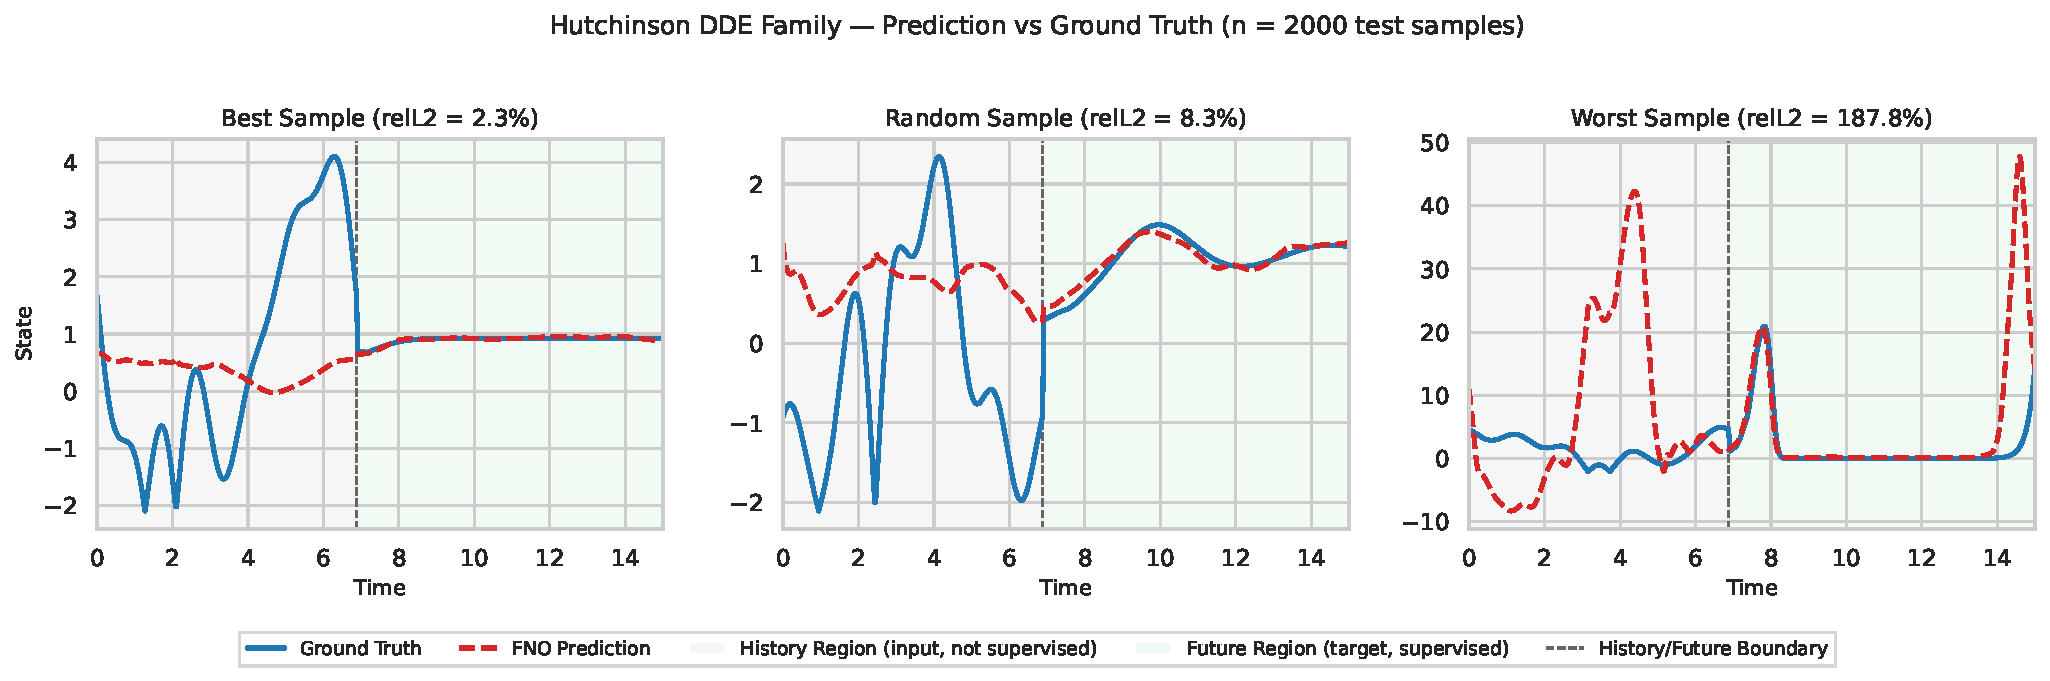
\includegraphics[width=\textwidth]{figures/hutch_hutch_with_regions.pdf}
  \caption{Hutchinson}
\end{subfigure}
\hfill
\begin{subfigure}[b]{0.48\textwidth}
  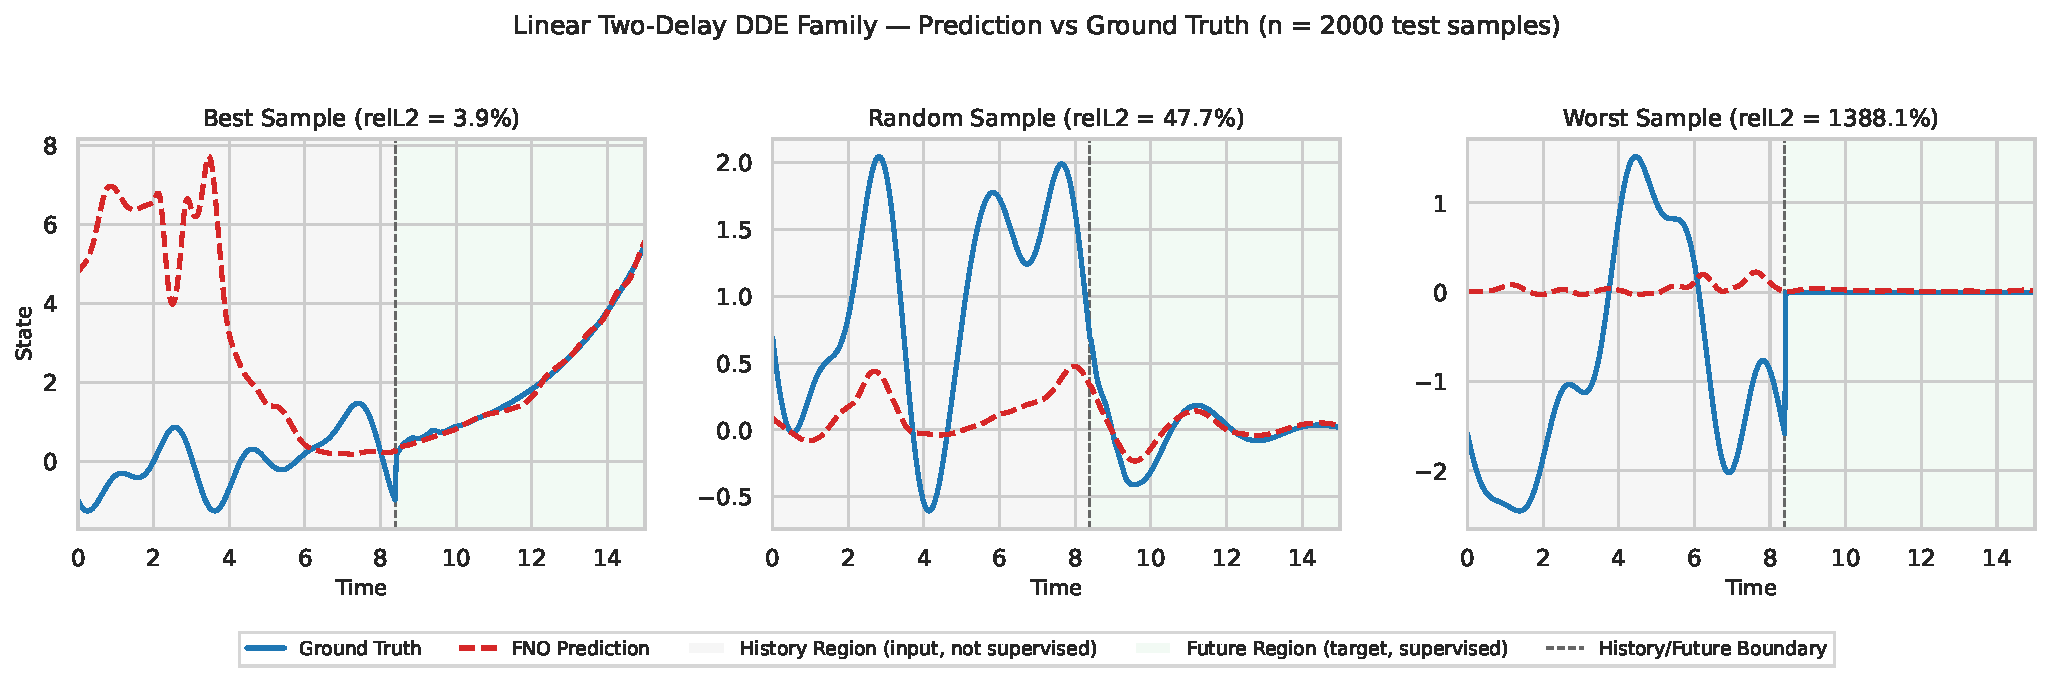
\includegraphics[width=\textwidth]{figures/linear2_linear2_with_regions.pdf}
  \caption{Linear2}
\end{subfigure}
\caption{Sample predictions with history (shaded) and future (white) regions.
Solid: ground truth; dashed: FNO prediction.}
\label{fig:predictions}
\end{figure}

% ------------------------------------------------------------------
\subsection{Out-of-Distribution Generalization}

Table~\ref{tab:ood-gaps} summarizes the OOD generalization gaps, defined as
the ratio of OOD median error to ID median error.  Larger gaps indicate worse
generalization.

\begin{table}[h]
\centering
\caption{Out-of-distribution generalization gaps (OOD median / ID median).
Higher values indicate worse generalization.}
\label{tab:ood-gaps}
\begin{tabular}{lccc}
\toprule
Family & OOD-delay & OOD-history & OOD-horizon \\
\midrule
Hutchinson  & 7.0$\times$ & 2.4$\times$ & 4.1$\times$ \\
Linear2     & 1.5$\times$ & 1.6$\times$ & 2.8$\times$ \\
Van der Pol & 2.6$\times$ & 4.0$\times$ & 4.3$\times$ \\
DistUniform & 5.1$\times$ & 11.3$\times$ & 2.4$\times$ \\
DistExp     & 4.2$\times$ & 3.9$\times$ & 1.5$\times$ \\
\bottomrule
\end{tabular}
\end{table}

\paragraph{OOD-delay.}
Extrapolation to unseen delay values produces the largest gaps for Hutchinson
(7.0$\times$) and DistUniform (5.1$\times$).  This is expected: the delay
$\tau$ directly controls the oscillation period in these families, so unseen
delays produce qualitatively different dynamics.  Linear2 shows a smaller gap
(1.5$\times$), likely because its difficulty is already high in-distribution.

\paragraph{OOD-history.}
Switching from Fourier-series histories (training) to cubic-spline histories
(test) reveals that models partially memorize the history function class.
DistUniform is most affected (11.3$\times$), suggesting the distributed-delay
averaging amplifies sensitivity to the smoothness structure of the input.

\paragraph{OOD-horizon.}
Extended prediction horizons ($T = 20$ vs.\ $T = 15$) generally produce moderate
gaps (1.5--4.3$\times$).  DistExp shows the smallest gap (1.5$\times$), as its
exponential kernel damps long-range dependencies.

Figure~\ref{fig:error-vs-time} shows the error-vs-time curve for Hutchinson across
all test splits, illustrating how errors accumulate over the prediction horizon and
diverge under distribution shift.

\begin{figure}[h]
\centering
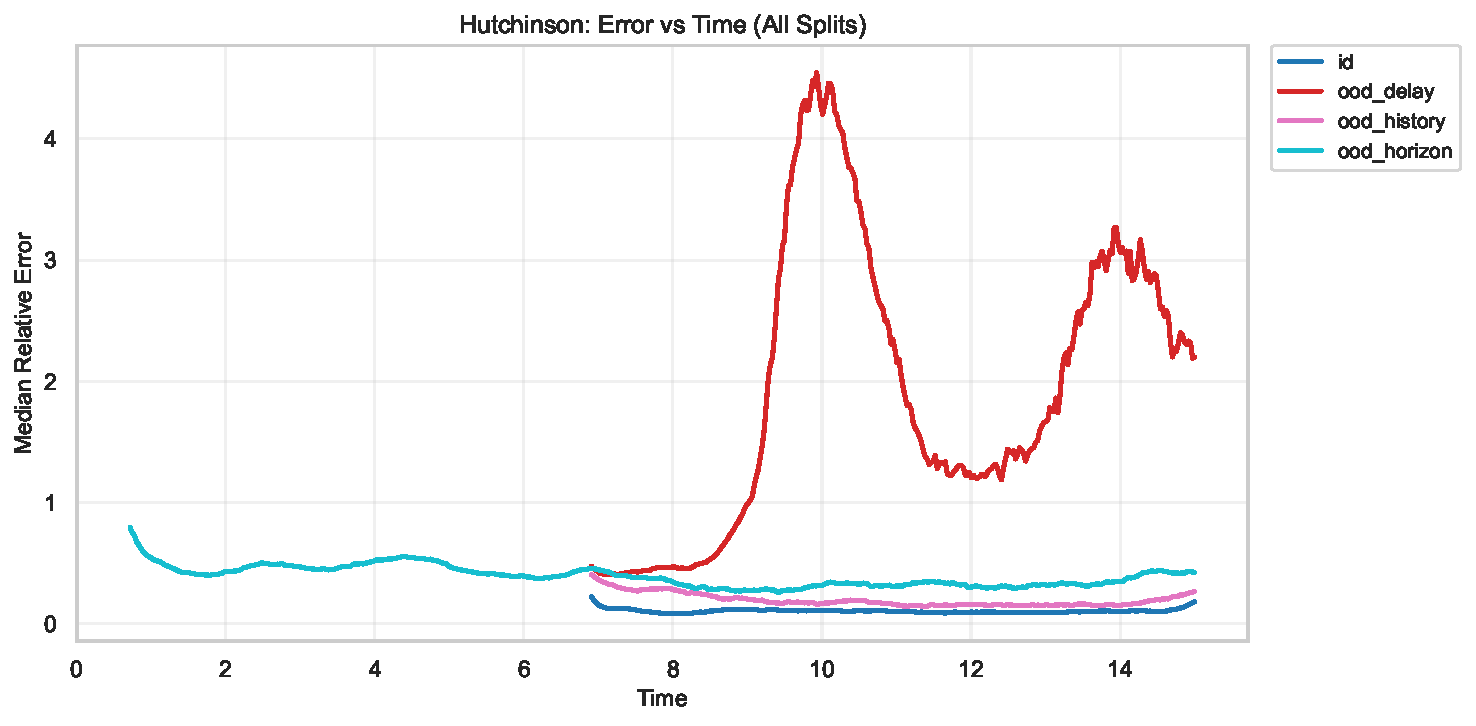
\includegraphics[width=0.65\textwidth]{figures/hutch_error_vs_time_all_splits.pdf}
\caption{Relative $L^2$ error vs.\ time for the Hutchinson family across ID and OOD
test splits.  Errors grow with prediction horizon and are amplified under distribution shift.}
\label{fig:error-vs-time}
\end{figure}

% ------------------------------------------------------------------
\subsection{Temporal Error Structure}

To understand how prediction quality degrades over time, we partition the
prediction horizon into three segments: Early $[0, 3.75]$, Mid $[3.75, 11.25]$,
and Late $[11.25, 15]$.  Table~\ref{tab:time-segments} reports the median
error in each segment.

\begin{table}[h]
\centering
\caption{Median relative $L^2$ error by time segment (ID test).}
\label{tab:time-segments}
\begin{tabular}{lccc}
\toprule
Family & Early & Mid & Late \\
\midrule
DistExp     & $<$0.001 & 0.034 & 0.022 \\
DistUniform & $<$0.001 & 0.047 & 0.049 \\
Hutchinson  & $<$0.001 & 0.063 & 0.102 \\
Van der Pol & $<$0.001 & 0.077 & 0.153 \\
Linear2     & $<$0.001 & 0.242 & 3.088 \\
\bottomrule
\end{tabular}
\end{table}

All families achieve near-zero error in the early segment, where the solution
is most constrained by the history function.  Errors grow monotonically for most
families, with Linear2 exhibiting a dramatic late-time blowup (mid: 0.24 $\to$
late: 3.09), indicating that the two interacting delays create compounding error
dynamics.  Notably, DistExp shows a slight \emph{decrease} from mid to late,
consistent with its exponential kernel damping long-range dynamics.

% ------------------------------------------------------------------
\subsection{Discussion}

Several patterns emerge from the baseline experiments:

\paragraph{Difficulty correlates with delay structure.}
Distributed delays (DistExp, DistUniform) are consistently easier than discrete
delays (Hutchinson, Van der Pol), which are in turn easier than multi-delay
systems (Linear2).  The integral averaging in distributed delays smooths the
operator's dependence on past states, producing a more regular input--output
mapping that is easier for the FNO to approximate.

\paragraph{The FNO's global receptive field is well-suited for delay dynamics.}
Unlike local methods (e.g., finite differences), the FNO's spectral convolution
captures long-range temporal dependencies in a single layer.  This is particularly
advantageous for DDEs, where the solution at time $t$ depends on values at $t - \tau$
that may be far away in the discretized sequence.  The 4.6--31.8$\times$ improvement
over the naive baseline confirms that the FNO learns meaningful delay structure.

\paragraph{OOD-history gaps reveal memorization of the history class.}
The large gaps under history distribution shift (up to 11.3$\times$ for DistUniform)
suggest that models partially memorize the smoothness properties of the Fourier-series
training histories rather than learning the underlying delay operator.  This motivates
training with diverse history function classes.

\paragraph{Multi-delay interactions remain challenging.}
Linear2's high ID error (0.612) and dramatic late-time blowup indicate that
the interaction of two delays $\tau_1$ and $\tau_2$ creates dynamics that are
fundamentally harder to approximate.  The FNO must implicitly learn the coupled
characteristic equation structure, which may require greater model capacity or
specialized architectures.

\subsection{Scope of the frozen baseline vs.\ extended benchmark}
\label{sec:scope-frozen-vs-phase-b}

The experiments reported in this section constitute the \emph{frozen
baseline}: a single FNO1d-Residual model ($\sim$93k parameters)
evaluated on five families across four OOD splits and one data scale.
Numerical results are reproducible from the manifest
\texttt{freeze\_manifest\_all5\_v2.json} and the tag
\texttt{baseline\_all5\_frozen\_v2}.

The extended benchmark (Phase B, specified in
\texttt{configs/sweep\_phase\_b.yaml}) broadens the evaluation along
three axes simultaneously.  Along the \emph{model} axis, the
11-model zoo from the experimental design document is ported and
smoke-tested: PlainMLP, MLP with cyclic-shift augmentation at two
budgets, FNO1d, DeepONet, MemNO, ANIE, LocalizedNO, LNO, MFNO, LEMO,
and LEMO$_{\sigma}$($\sigma = 0.9$).  Along the \emph{family} axis,
VdP and DistUniform are added and (pending data generation)
Mackey--Glass and Predator--Prey.  Along the \emph{split} axis,
continuous-$\tau$ evaluation is added for the three families where the
continuous-lag equivariance theorem is the most natural operational
story (DistExp, DistUniform, Hutchinson), and history-amplitude
evaluation for the three families most sensitive to initial-condition
magnitude (VdP, Mackey--Glass, Predator--Prey).  The full matrix is
$(7~\text{families}) \times (\text{applicable splits}) \times (12~\text{model entries}) \times (3~\text{seeds})
= 972~\text{runs}$, matching the plan's $\sim$700-run estimate after
dedup.  Results from this sweep will be reported in a revised version
of this section once the Mackey--Glass and Predator--Prey generators
and the continuous-$\tau$ off-grid data pipeline are available.


\section{Conclusion}
% Conclusion

We have presented an operator learning framework for delay differential equations
using Fourier Neural Operators.  Our contributions include: (i) a benchmark suite
of five DDE families spanning discrete and distributed delays, (ii) a robust data
generation pipeline with quality control and reproducibility guarantees, and
(iii) baseline experiments demonstrating the feasibility and current limitations
of FNO-based operator learning for DDEs.

The baseline FNO achieves 4.6--31.8$\times$ improvement over naive persistence across
all families, with median relative $L^2$ errors ranging from 0.077 (DistExp) to 0.612
(Linear2).  The difficulty ranking---distributed delays easiest, multi-delay systems
hardest---provides a useful guide for future architecture development.  Out-of-distribution
experiments reveal that generalization to unseen delay values and history function classes
remains a significant challenge, with gaps up to 7$\times$ and 11$\times$ respectively.

\paragraph{Limitations.}
Our baseline uses a single architecture (93k-parameter FNO) without per-family
hyperparameter tuning.  The benchmark currently covers five families; while these
span the major DDE categories, state-dependent delays and neutral-type DDEs are
not yet included.  The OOD splits test one axis of variation at a time rather than
joint shifts.

\paragraph{Future work.}
A scaling study across model sizes (small/medium/large), dataset sizes
(2k/10k/50k), and additional families (including neutral DDEs, chaotic
Mackey--Glass variants, and stiff Van der Pol systems) is currently underway.
Other promising directions include: comparison with alternative operator learning
architectures (DeepONets, Transformers), training with mixed history function
classes to improve OOD robustness, and extending the framework to
state-dependent and time-varying delays.

\paragraph{Three-phase benchmark extension.}
The follow-on benchmarking effort is structured in three phases.
\emph{Phase~A} (theorem-verification suite) runs three small controlled
targets---continuous-lag toy, expansive linear delay, contractive
tanh delay---against PlainMLP, MLP with cyclic-shift augmentation at
multiple budgets, LEMO, and an LEMO$_{\sigma}$ ablation, in order to
verify directly the continuous-lag equivariance theorem, the
augmentation covering-radius lower bound, and the LEMO$_{\sigma}$
rollout-stability corollary.  \emph{Phase~B} (core DDE benchmark)
evaluates the 11-model zoo listed in Section~\ref{sec:scope-frozen-vs-phase-b}
across seven families (DistExp, VdP, Hutchinson, Mackey--Glass,
Predator--Prey, DistUniform, Linear2) and four evaluation splits
(in-distribution, lag-shift OOD, horizon OOD, and either
continuous-$\tau$ OOD or history-amplitude OOD depending on family),
stratified by a lag-dependence strength score (LDS) to distinguish
lag-dominant from weakly lag-dependent regimes.  \emph{Phase~C}
(stability deep-dive) sweeps $\sigma \in \{0.5, 0.7, 0.9, 0.99, \text{unconstrained}\}$
on three representative families to characterize the
accuracy--stability frontier of the LEMO$_{\sigma}$ certified subclass.
The scaffolding for Phase~B is committed
(\texttt{configs/sweep\_phase\_b.yaml},
\texttt{slurm/sweep\_phase\_b.py}); the remaining blockers are
data generation for Mackey--Glass and Predator--Prey, and an
off-grid continuous-$\tau$ data pipeline.


\bibliographystyle{plainnat}
\bibliography{references}
\end{document}
